\documentclass{standalone}
\usepackage{tikz}

\begin{document}
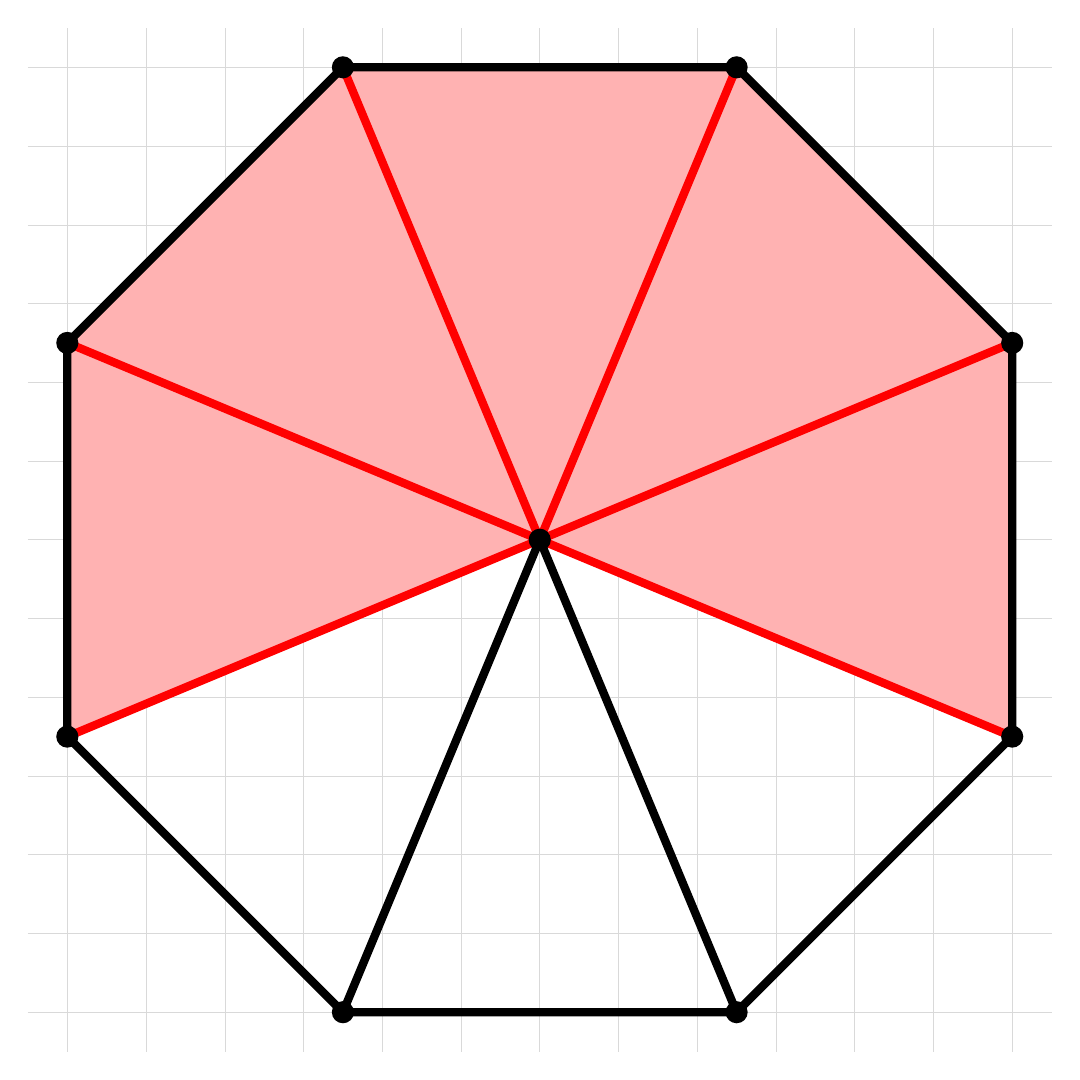
\begin{tikzpicture}

   \coordinate (Center) at (0,0);
   \coordinate (A1) at (-6,2.5);
   \coordinate (A2) at (-2.5,6);
   \coordinate (A3) at (2.5,6);
   \coordinate (A4) at (6,2.5);
   \coordinate (A5) at (6,-2.5);
   \coordinate (A6) at (2.5,-6);
   \coordinate (A7) at (-2.5,-6);
   \coordinate (A8) at (-6,-2.5);

   %\node at (Center) {\includegraphics[width=1.025\textwidth]{004.png}};


   \draw[step=1cm,gray!30,very thin] (-6.5,-6.5) grid (6.5,6.5);

\fill[line width=3pt,color=red!30] (Center) -- (A8) -- (A1) -- (A2) -- (A3) -- (A4) 
                            -- (A5) -- (Center);

   
   \draw[line width=3pt] (A1) -- (A2) -- (A3) -- (A4) -- (A5) -- (A6) -- (A7) -- (A8) -- (A1);

\draw[line width=3pt,color=red] (Center) -- (A1);
\draw[line width=3pt,color=red] (Center) -- (A2);
\draw[line width=3pt,color=red] (Center) -- (A3);
\draw[line width=3pt,color=red] (Center) -- (A4);
\draw[line width=3pt,color=red] (Center) -- (A5);
\draw[line width=3pt] (Center) -- (A6);
\draw[line width=3pt] (Center) -- (A7);
\draw[line width=3pt,color=red] (Center) -- (A8);


   \fill (Center) circle (4pt); % node[color=red,below] {(Center)};
   \fill (A1)     circle (4pt); % node[color=red,below] {(A1)};
   \fill (A2)     circle (4pt); % node[color=red,below] {(A2)};
   \fill (A3)     circle (4pt); % node[color=red,below] {(A3)};
   \fill (A4)     circle (4pt); % node[color=red,below] {(A4)};
   \fill (A5)     circle (4pt); % node[color=red,below] {(A5)};
   \fill (A6)     circle (4pt); % node[color=red,below] {(A6)};
   \fill (A7)     circle (4pt); % node[color=red,below] {(A7)};
   \fill (A8)     circle (4pt); % node[color=red,below] {(A8)};

    
\end{tikzpicture}



\end{document}